\documentclass[12pt,a4paper,oneside,openany]{book}

\usepackage{xcolor}
\usepackage{minted}
\usepackage[utf8]{inputenc}
\usepackage{tikz}
\usepackage{caption}
\usepackage{gensymb}
\usepackage{lmodern}
\usepackage{multirow}
\usepackage{booktabs}
\usepackage{array}
\usepackage{adjustbox}
\usepackage{upquote}
\usepackage{amsmath}
\usepackage{titlesec}
\usepackage[hidelinks]{hyperref}
\usepackage{fancyhdr}
\usepackage{wrapfig}
\usepackage{graphicx}
\usetikzlibrary{mindmap,shadows, shapes, arrows, positioning}

\newcommand{\projecttitle}{Fabrik - an e-commerce web application}
\newcommand{\projectauthor}{Niema Attarian \\[0.2cm] Mark Gill}
\newcommand{\projectadvisor}{Dr John Healy and Gerard Harrison}
\newcommand{\projectprogramme}{B.Sc.(Hons) in Software Development}
\newcommand{\projectdate}{\today}




\tikzstyle{rect} = [rectangle, fill=blue!50, text width=4.5em, text centered, minimum height=4em, rounded corners]
\tikzstyle{line} = [draw, ->, very thick]
\tikzstyle{oval} = [ellipse, fill=green!50, text width=5em, text centered]

\newcolumntype{x}[1]{>{\centering\arraybackslash\hspace{0pt}}p{#1}}


\begin{document}
  \begin{titlepage}
    \begin{minipage}[t][6cm]{\textwidth}
      \centering
      \rule{\linewidth}{0.5mm} \\[0.4cm]
      { \LARGE \bfseries \projecttitle \\[0.4cm] }
      \rule{\linewidth}{0.5mm} \\[0.8cm]
    \end{minipage}
    
    \begin{minipage}[t][6.5cm]{\textwidth}
      \centering
      \textbf{\projectauthor}\\[0.5cm]
      \projectprogramme
    \end{minipage}
  
    \begin{minipage}[t][1cm]{\textwidth}
      \centering
      \textsc{\projectdate}
    \end{minipage}
      
    \begin{minipage}[t][3cm]{\textwidth}
      \centering
      \textbf{Final Year Project}\\[0.3cm]
      Advised by: \projectadvisor \\[0.1cm]
      Department of Computer Science and Applied Physics\\
      Galway-Mayo Institute of Technology (GMIT)
    \end{minipage}
  
    \begin{center}    
      
\includegraphics{img/gmit-logo.jpg}
    \end{center}
  \end{titlepage}
  \setcounter{page}{2}
  \tableofcontents
 
  %!TEX root = project.tex

\listoffigures

\chapter*{About this project}
\paragraph{Abstract}
Online shopping is becoming one of the fastest growing markets ever. It is used by people on an almost day-to-day basis, allowing them to purchase any product they wish by just a click of a button. Many retail companies are creating online web applications to broaden their target market and in-turn potentially increasing sales. This leads to increasing competition and a race to who can maintain their audience by re-vamping their websites to appeal to their audiences and provide more products quickly.

In this project, we aim to develop a fully functioning and aesthetically pleasing e-commerce web application. Our objective is to keep it simple; have a clean looking web page that maintains its full functionality with relevant security.

\paragraph{Authors}
This final year project was designed and built by Mark Gill and Niema Attarian, final year students of Software Development attending Galway-Mayo Institute of Technology.

\chapter{Introduction}
Over the course of our first three years studying software development in G.M.I.T., we have learned an extensive range of programming languages, frameworks and platforms. These three years had left us ready and prepared to put into practise what we learned for our final year project.

In the beginning of our final year we were presented with our final year group project worth 15 credits over the course of two semesters. Taking what we have learned over our first three years, and a few weeks of brainstorming ideas, we came to a mutual agreement on an idea which we would implement as part of our project. This idea was further discussed with our project supervisors, outlining whether it was worthy as a level 8 project and what criteria to meet along the way.

This chapter will outline the basis of what will further be discussed in this dissertation. We will start by outlining the main objectives we aim to meet throughout our project and dissertation, discuss the metrics of failure and success of a project and break down what each chapter of the dissertation will include.

\section{Objectives of the project}
The objective we set out to accomplish in this project was to put in place what we learned over the previous three years into an e-commerce application. We planned on doing this using technologies we were familiar with and technologies we had little experience with. We did this to test our ability by adapting to various tasks presented to us. This approach was also done to increase our understanding of technologies unfamiliar to us.

This project was divided into two parts; a detailed minor dissertation and an applied project. Below, each part is broken down into the objectives we set out to achieve. 

The objectives for the dissertation are as follows;
\newline
\newline
\textbf{Dissertation}
\begin{itemize}
  \item \textbf{\textit{Outline the basic concept}} We will discuss the concept of this project, diving in-depth into the inspiration behind the project and why specific choices were made.
  \item \textbf{\textit{Understand the technologies used}} The availability of technologies to use when creating an e-commerce application has grown significantly over the years and is ever expanding. We will explore all the possible options of technologies we could've used outlining the pro's and con's of them and justifying our choice.
  \item \textbf{\textit{Detail of the development of the project}} This dissertation plans to give a comprehensive guide of the development of our applied project from start to finish. This is achieved by breaking down our project and examining each step taken.
\end{itemize}
The objectives for the applied project are as follows;
\newline
\newline
\textbf{Applied Project}
\begin{itemize}
  \item \textbf{\textit{Implementing and exploring new and existing technologies}} It is important that throughout this project we implemented new technologies while still improving on existing one we have already worked with. This helps in increasing our learning outcome by expanding our skill-set.
  \item \textbf{\textit{Aesthetic and simple website}} Design a simple and easy to use website was very important when planning our objective. It is essential that we design a user friendly site which is easily navigable and customizable.  
  \item \textbf{\textit{Collaborative effort amongst teammates}} This dissertation will detail the importance of collaboration in project. As a team it is important to communicate and co-operate effectively and in this dissertation we will go through how we divided up work equally and how it worked together.
\end{itemize}

\subsection{Metrics for success and failure}
A key component in designing and building a project is providing metrics or standards that the creators aim to achieve to determine whether the project was a success or a failure. In doing so, it can also set focus to what the primary goal is without getting side-tracked. A breakdown of the metrics of this project have been outlined below.

\subsubsection{Applied project which is fully functional and simple to use}
It was imperative that in measuring the success or failure of our project, we outline requirements that are to be met when in development. These requirements can be viewed in \textit{Chapter 1, Section 1.1.2} of this dissertation. Here, we outlined what the minimum functioning components of an e-commerce application should be while ensuring that it is easy to use by any user. 

\subsubsection{A detailed, comprehensive minor dissertation} It was necessary that with a functioning project came a dissertation that was comprehensive and easy to read. This included breaking down the project into chapters, detailing the background of project and the methods put into place. These methods included evaluating the technologies used and how they were implemented effectively.

\subsubsection{Collaboration as a team}
We felt a major aspect in measuring success or failure in a project was determining how well each member of the team could collaborate with one another. This involves the availability of each member, how open each member was to new ideas or changes to the project, the willingness to listen and communicate to one another and how issues were approached and resolved. 

\subsection{User requirements of the project}
In developing this project, we discussed amongst ourselves and our project supervisor what specific user requirements were necessary for an online commercial clothing website. Below is a list of user requirements agreed upon and implemented.
\newline
\newline
\newpage
\textbf{Requirements:}
\begin{itemize}
  \item Must be able to register a user.
  \item Must be able to log in and log out.
  \item Log in must carry across each page.
  \item User can select an item to view on a item details page
  \item User can add items to the cart
  \item User can remove items from cart
  \item User can view their details on a profile page
  \item Must be able to edit user details
\end{itemize}

\section{Breakdown of each chapter}
This dissertation is broken down into different required chapters. Each chapter contains different aspects of the project in great detail. The following sub-sections detail what each of these chapters are and what they entail.

\subsection{Context}
Context, chapter 2, discusses why the idea was chosen for this project. This chapter also goes into further detail the background, environment and setting of our idea.

\subsection{Methodology}
In methodology, chapter 3, we will describe the procedures of how we went about doing our project. This involves what planning was put in place, how we organised, managed and developed this project. We will briefly describe the the various technologies, frameworks and platforms chosen and why they we chosen over others.

\subsection{Technology Review}
Technology review, chapter 4, will outline the technological aspect of the project. This includes a breakdown, in depth, of each of the technologies used at a conceptual level. It will describe how these technologies were implemented and why a specific technology was chosen over another.

\subsection{System Design}
System design, chapter 5, describes the how of the project. We will detail the components of the projects and why we implemented each of them. Furthermore, these components will be described in detail with aid of diagrams and screenshots.

\subsection{System Evaluation}
In system evaluation, chapter 6, will outline the robustness of our project. This was done through testing using frameworks such as Selenium which we were familiar with. Also expressed in this chapter is the scalability of this project. A run down of what could possibly be improved in the project and all the limitations we faced in building it.

\subsection{Conclusion}
Finally, the conclusion will briefly review the goals and objectives initially set out in this dissertation and discussing how these objectives were achieved. Furthermore, the measure of success or failure will be outlined given the overview of what has been implemented in this project.

\section{GitHub Repository}
As this project was a collaborative effort, each member agreed that GitHub would be an adequate version control. GitHub is a development platform allowing users to host and review code and work in a collaborative manner. The benefits of this platform is discussed in great detail in \textit{Chapter 3, Methodology}. Our project repository can be found in our appendices chapter under both providing both Niema's and Mark's repositories. A README.md is available on the main page of each repository providing instructions on how to clone/download the project, the requirements of the project and how to run the project successfully.

\chapter{Context}

Online shopping has grown drastically over the past two decades. Since the introduction of the World Wide Web the consumer use became a possibility which created a promising market for retailers. In 1995, retailers like Amazon and eBay were introduced to the online market. Amazon launched initially as a as an online book seller. It was considered to arguably be the online market maker which paved the way for online shopping in years to come\cite{openlearn_2019}. The launch of eBay was also influential for the online market industry as, like Amazon, they created a platform for the sale of items online which eventually introduced an auctioning system into the mainstream commercial websites we see today.

\section{Context of the project}
Our decision to plan and build a commercial clothing website was largely influenced by many well known clothing sites such as ASOS, Depop and JD Sports. These websites attract millions of consumers worldwide. The success of these sites are essentially down to the wide availability of the site and the items they sell, the simple aesthetic of each of these websites and the scalability of each of these sites. Over time, they are open to the change in demand from consumers which can change rapidly in today's climate. 
\newpage
\subsection{Business Model}

Although many commercial sites can very between consumer-to-consumer like Depop, business-to-consumer like JD Sports or both consumer/business-to-consumer like ASOS, we decided that our best approach would be a business-to-consumer project. The reasoning behind this choice was based on research we did into the differences between these business models and found many appealing advantages to the business-to-consumer model. With these advantages, however, came some challenges involved with this model.

\subsection{Capabilities of the Business-to-Consumer model}
\paragraph{Availability}One of the most appealing advantages is the ability to provide a product to the consumers in real-time. Essentially a product provided by a company of this type is available 24 hours a day, 7 days a week 365 days a year. This includes customization of goods to match the varying demands of a market\cite{santosh_2015}.

\paragraph{De-Intermediation}This aids in eliminating the so called 'middle-man' between a manufacturer and consumer offering a simple distribution and differentiation based on consumer needs aiding in potential costs and profits\cite{santosh_2015}.

\paragraph{Collaboration}This aids in collaborating with other parties to help further the business. An example of this may include integrating a payment API such as PayPal or Venmo. This can help ensuring a greater deal of security and supporting real-time exchange of consumer information\cite{santosh_2015}.

\subsection{Challenges of the Business-to-Consumer model}
\paragraph{Redesign of business}Although very adaptable as previously discussed, with a varying demand among consumers and strong competition comes a constant redesign of the business. This can range from the products being sold down to the ergonomics of the website itself. To become a successful business re-designing must be well implemented on every scale.

\paragraph{Matching technology to business needs}A major problem many business-to-consumer companies face is that of matching the technological needs of a business. This comes with a rapidly expanding market where technologies are adapting at enormous rates and this problem is exasperated further by the flood of new products to a market. 

\chapter{Methodology}
This chapter will detail the approach and procedures we took to complete this project. This includes the planning, meetings, management and organisation that was put in place by us and our advisors to tackle this project effectively. Furthermore, this chapter will also outline the various technologies that we reviewed and agreed upon for our project. Finally, we conclude this chapter detailing the type of testing we proposed would fit the project.

Initially, when this project began with three members, we discussed how we would break down our idea both between us and with our project supervisor. Our first idea consisted of a commercial Angular application, similar to that of a business to consumer application like Amazon or eBay. Our idea consisted of a front-end, back-end, a neural network which took in a picture that identified a particular product like shoes, a t-shirt, etc and the cloud hosting. Along with advice from our supervisor,  we agreed on sharing the responsibility of the project as equally as possible with Niema designing the front-end of the application, Mark coding the back-end of the application, Richard in charge of the neural network and the cloud hosting being a final addition towards the end of this project.

We met two-to-three times as week as a group to discuss our approach and any issues we had. We also routinely had weekly meetings, on a Monday morning, with our supervisor Gerard to discuss ideas, frameworks and various methods on how to approach this project. We would detail our progression in these meetings with Gerard and also mention any outstanding issues.
We kept a very open mindset in developing our project. This was clear in our idea choice. It was extremely versatile which helped with any suggested changes or approaches which differed from our base idea. 

However, as the weeks continued and further discussion with our supervisor, we mutually agreed that our idea and workload was not sufficient for a three person group. Therefore, we disbanded into a two-person group of Niema and Mark. Following the advice of our supervisor, we discussed how we would restructure our project and re-assign the workload evenly. The scope of the project barely changed with the only difference being the removal of the neural network aspect. We did, however, decide to change the language we planned on developing the application from Angular to Django.

\section{Incremental and iterative approach to the development}
It was important from a project management perspective to establish an effective approach to this project. These approaches ranged from traditional, agile and waterfall. Research into each of these approaches was key to determine which suited our project given the time scale we were given and how the work was divided. 
We agreed that our choice must be adaptable and straight-forward to create a positive collaborative working environment going forward.

\subsection{Scrum}
\begin{wrapfigure}{r}{2.9in}
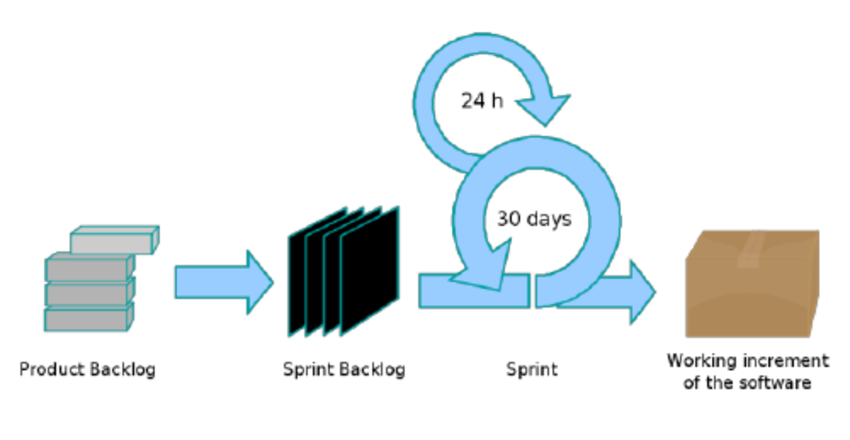
\includegraphics[scale=0.25]{img/Diagram-of-Scrum-agile-method-13.png}
\caption{Scrum process diagram \cite{inproceedings}}
\end{wrapfigure}
The approach we believed that was best suited in successfully completing our project was a Scrum approach. The Scrum approach is a software development process for smaller teams which suited us best having going from a three person team to a two person team. The breakdown of Scrum was simple to understand and put in place for this project. Like all project, the initial stage of this approach was the planning phase. This involved gathering each member and developing a structure for this project and a leading member. Mark Gill was chosen to be our project leader. His role was to outline a definitive and flexible approach broken up into what could be considered as sprints\cite{rising2000scrum}.

Sprints are short set time period in which allocated work from a project leader is completed. This work should be ready for review by the next scrum meeting. These meeting were planned and agreed upon by each member. We agreed that Monday would be a good time slot for our Scrum meeting where we reviewed work that was set out and planned for our next sprints. This day of the week was deemed to be the most optimum day as not only was it the same day as our meeting with our project supervisor, but it allowed for straightforward planning for other work we had in place from other modules for the upcoming college week. The sprints proved very effective in dividing up the work into smaller segments and setting time-frames to achieve these segments\cite{rising2000scrum}.

\section{Selection criteria for Technologies, Frameworks and Platforms}
Selecting the correct technologies, frameworks and platform was key in creating a successful project. We had to ensure that what we were choosing fitted our project spec and could be implemented effectively. This selection will give a brief overview of what we chose and how we went agreeing on our choices. The technologies, frameworks and platforms are discussed in further detail in \textit{Chapter 4, Technology Review}. The sub-sections below will briefly outline our approach to using these technologies.
\subsection{Technologies}
\paragraph{TypeScript}
Our initial approach included using TypeScript[1] to build our commercial application. We believed that this language was best suited for our project as it is essentially super-set of JavaScript, a language we are familiar with and have used consistently over our four years of software development. It has the ability to enable easier development on a large scale which was essential to our versatile and expandable idea\cite{bierman_abadi_torgersen_2014}.

\paragraph{Python}
When our group disbanded from three members to two members, our idea of initially using TypeScript had changed. We decided upon using a language that we had the least experience in and that language being Python. Python is a language we had the short end of two semesters using, so we believed that in using it for our final year project, it would've been a great learning curve. It is an ever growing language becoming very popular in web development so we confident that it was the correct choice in switching from TypeScript.
\newpage
\paragraph{HTML}
HTML was agreed upon for the front-end of the project. This choice was made mainly for it's simplicity. It is easily implemented and designed. We have had experience with this markup language since the beginning of college and we figured it would be best fitted for your main web-page being very versatile with other frameworks and platforms.

\paragraph{CSS}
CSS was agreed upon for the design of the front-end of the project. It is considered the skin of a web-page. It goes hand in hand with HTML and is extremely easy in integrating design for it. As previously mentioned, years of practise and use has been put into CSS throughout the course of our college experience with our other projects. We believed that putting this experience into use would results in a clean looking project.

\paragraph{JavaScript}
JavaScript was a fundamental choice in development of the project. It was essentially the core for some aspects of our web-page. A primary reason for the choice of this language was that it could integrate with CSS and HTML fluidly. These are said to hand-in-hand with one another when it comes to the development in any web-page so we deemed JavaScript to be essential.

\subsection{Frameworks}
\paragraph{Angular}
With our first development idea including TypeScript, we found that Angular to be the best framework for our large-scale, single page application. Angular was a familiar framework to us, one that we have used for the course of two years. Basic CRUD functionality was easily implemented in this framework which is why it was our initial choice for our project.

\paragraph{Django}
A change in our language came a change in framework in regards to development project. With Angular being a very good web-page oriented framework, we needed an equivalent when it came to Python. We found the Django framework worked best with Python and was the perfect alternative to angular as it was also a highly regarded web development framework. This framework is used widely amongst large websites and we believed that it would be a great framework to learn and adapt to as part of our project. 
\newpage
\subsection{Platforms}
\paragraph{GitHub}
As a team based final-year project, we unanimously agreed that GitHub\cite{github} would be best suited to manage our project. This decision was without hesitation as GitHub was used widely in our four years of studying Software Development. GitHub is widely used amongst every profession of software development and it is evident that the platform has helped improve the way in which software professionals work and collaborate\cite{zagalsky2015emergence}.

\section{What about validation and testing?}
Testing the application was very important to us. We wanted to ensure that it functioned smoothly and accurately. This will be detailed further in the dissertation in \textit{Chapter 6, System Evaluation}, where we breakdown the types of testing we put our project through to ensure it was of the standard and robustness we aimed to achieve.


\chapter{Technology Review}
This chapter will outline and breakdown each of the technologies that helped create and design this project. Each of these technologies will be discussed in detail on what they are, how they are implemented and why they were chosen over other alternative technologies.

\section{Framework}
\subsection{Django}
\begin{wrapfigure}{r}{1.9in}

\includegraphics[scale=0.35]{img/django.png}
\caption{Django}
\cite{fullstackpython}
\end{wrapfigure}
Django is a web framework developed in Python. The focus of Django is to make setting up your website as easy as possible. The framework is designed to get your application up and running rather quickly compared to other frameworks. This framework has many built-in components including HTML templates, admin panels and more. 
Django uses views and models to get the client side to connect with the server side. Models dictate the structure of the database itself and the views manipulate the data sent back from the HTML pages. It uses GETs and POSTs to return pages to the user or data to the server\cite{pythonforbeginners}.

We chose Django because we wanted to be able to use our skills in Python as we both enjoy using it. It has a lot of templates if needed, however, we may end up doing our own. We also feel the experience of a new framework to study would benefit us as we have worked with TypeScript and AngularJS many times before.

\section{Languages}
\subsection{HTML}
HTML (Hyper-Text Markup Language) is a language that makes use of tags to create web pages. These tags define which sections of the web page do what. These tags are only visible in the source code yet display cleanly on the web page when conducted correctly.

Here is an example of HTML:
\begin{figure}[h]
    \centering
    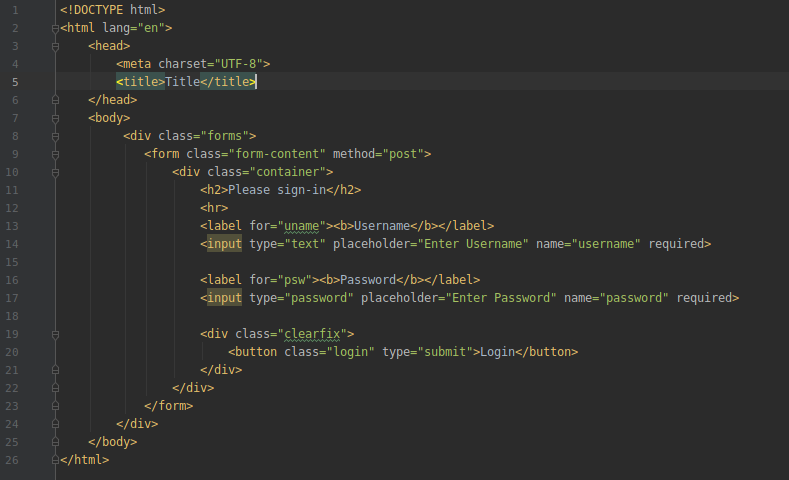
\includegraphics[scale=0.4]{img/htmlinput.png}
    \caption{HTML source code}
    \label{fig:my_label}
\end{figure}

Here is how the HTML is displayed:
\begin{figure}[h]
    \centering
    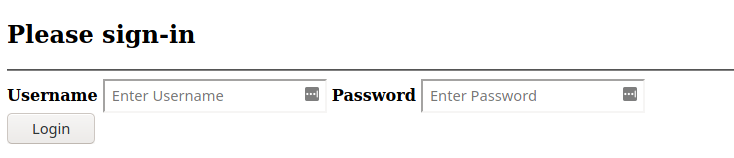
\includegraphics[scale=0.4]{img/htmloutput.png}
    \caption{HTML display page}
    \label{fig:my_label}
\end{figure}


We chose HTML as our web page display as it is extremely versatile and extensive. It is a language we have learned from our very first day of our first year of college along with CSS and JavaScript which are easily implemented with each other.
\newpage
\subsection{JavaScript}
JavaScript, along with HTML and CSS, is considered a core essential for web-page design and functionality. It is said to be the backbone of any web-page and is used widely by large companies such as Google.com, YouTube.com and Facebook.com \cite{w3techs}. JavaScript enables interactive web pages for the users by supporting event-driven functional programming styles such as API's.

As previously mentioned in the HTML sub-section, we chose JavaScript for our project as it was a core essential for the functionality of web-pages and a language we had extensive experience with throughout our college years. It enabled functionalities like our cart system in our project, something that will be detailed later in our dissertation.

\subsection{Python}
\begin{wrapfigure}{r}{2.05in}

\includegraphics[scale=0.25]{img/python.png}
\caption{Python}
\cite{python.org}
\end{wrapfigure}
Python is a high-level programming language which means it's more human-readable. It is considered by many to be one of the easier languages to learn. It has a very low of maintenance. It has an endless and ever-growing pool of great imports.
We chose Python because we had used it in other projects and we very much enjoyed our experience with it. We have used Python with Flask but not with Django.

\section{Database}
The database is extremely important to any application using one. There are many options and types out there so it is of the utmost importance to pick one that will make your development cycle as easy as possible. It is important to pick based on need for your specific application.
\newpage
\subsection{SQLite}
SQLite is a library used for relational database management. This doesn't require a separate server process to operate. This mean that the applications can interact directly with the SQLite database to read and write. SQLite is self-contained, meaning it doesn't need support from it's environment which makes it usable on a multitude of platforms like phones, tablets and consoles. It requires no configuration files since SQLite is server-less. SQLite is ACID(Atomic, Consistent, Isolated, Durable)-compliant. This ensures that writes to database are done fully or not at all.
We chose SQLite because we had learned from our research that it was by far the easiest to use with Django. It also benefits from being very durable and easy to understand and work with during the whole development cycle\cite{sqlite}. It's very fast and reliable. The concerns of scalability don't really affect us in this project.

\section{Styling the UI}
The styling of the user interface is essentially one of the most important aspects of a web-page. Its purpose is to allow users to navigate from page to page with great ease. It is also imperative that the design is easy on the eyes of the users while still maintaining their interests by using standout colours or styles. These styles can target certain audiences in different ways. Primarily speaking, how a web-page is designed impacts how an audience will perceive a brand comparing to other competing brands.

\newpage
\subsection{CSS}
CSS (Cascading Style Sheets) is primarily used to present and design markup languages like HTML. This design is achieved through improving the colours, fonts and the overall layout of a web-page.

Here is an example of a web-page with no CSS styling:

\begin{figure}[h]
    \centering
    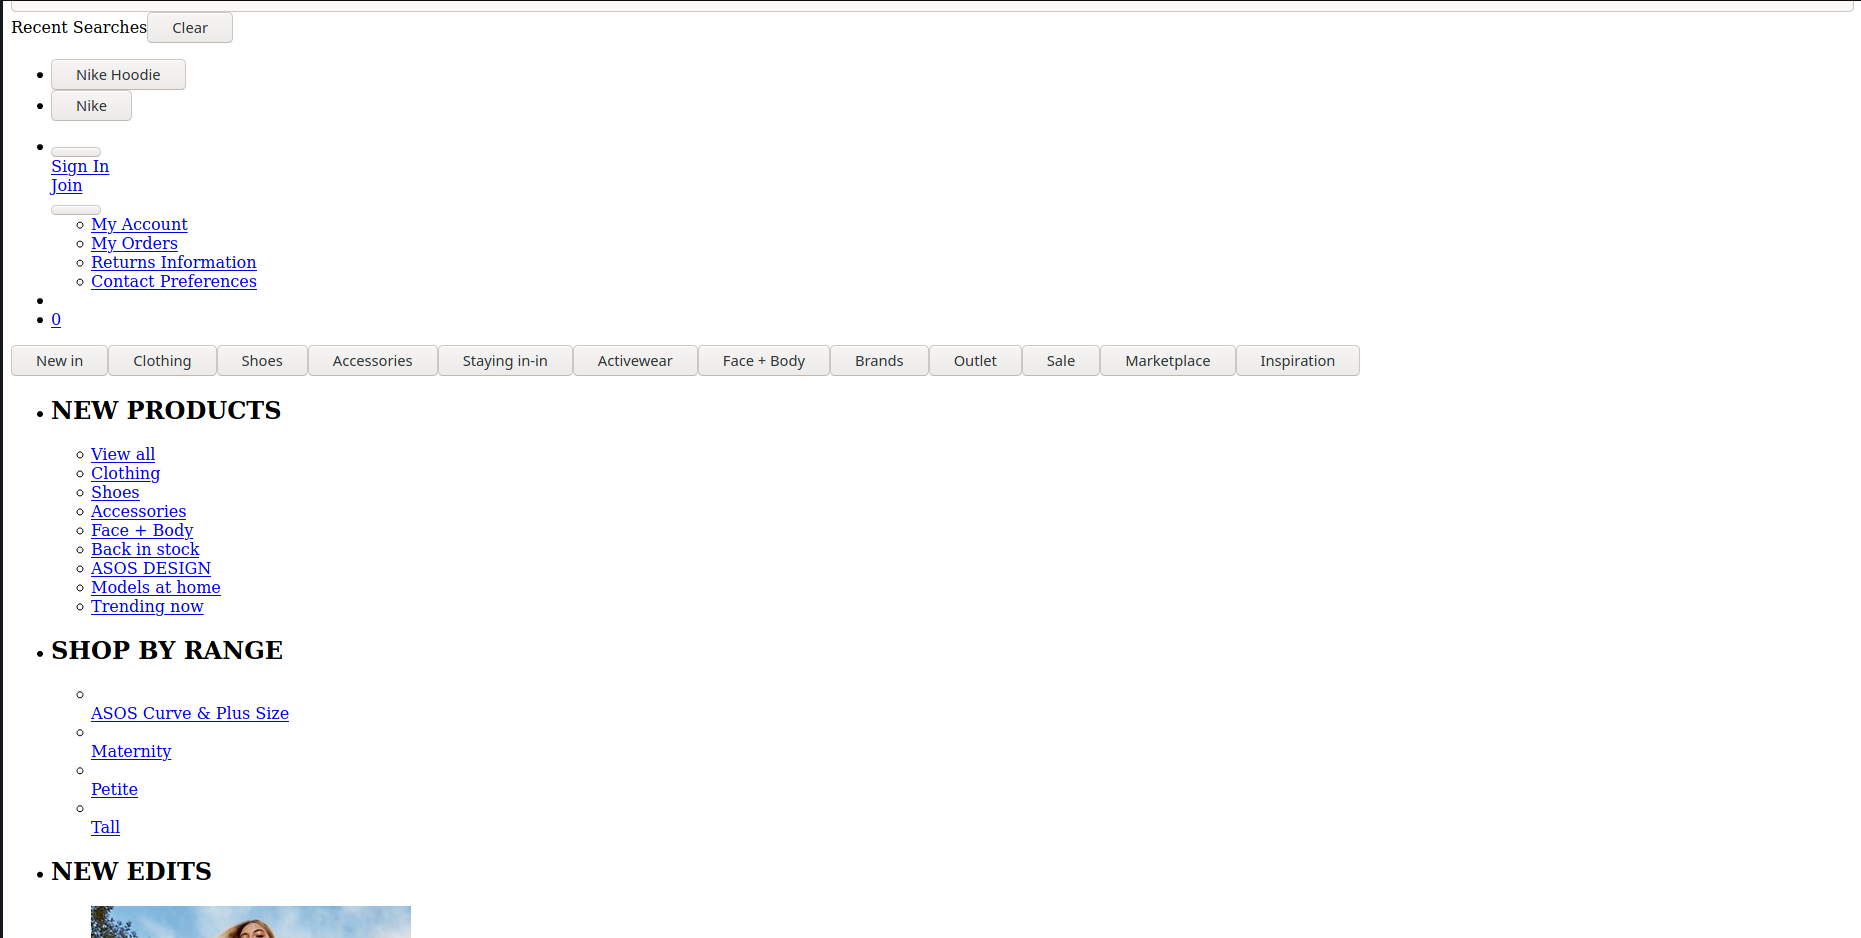
\includegraphics[scale=0.2]{img/nocss.png}
    \caption{ASOS web-page containing no CSS}
    \label{fig:my_label}
\end{figure}

Here is the same web-page containing CSS styling:

\begin{figure}[h]
    \centering
    
\includegraphics[scale=0.2]{img/withCss.png}
    \caption{ASOS web-page containing CSS}
    \label{fig:my_label}
\end{figure}
\newpage
As previously discussed in methodology, CSS was chosen for our project due to its simplicity. Along with HTML, it is a style-sheet-language we have had years of experience with and believed in using it, it would achieve our goal of an aesthetic e-commerce website.

\subsection{LaTeX}
LaTeX is a document preparation system. As opposed to the likes of Microsoft word and other word processors, LaTeX uses mark-up tags to create the structure of a document. Similarly to HTML, these tags are only visible in the source code of the document whereas it produces a a clean and concise display of the document when done correctly.

LaTeX tags are shown in this image of the source code.

\begin{figure}[h]
    \centering
    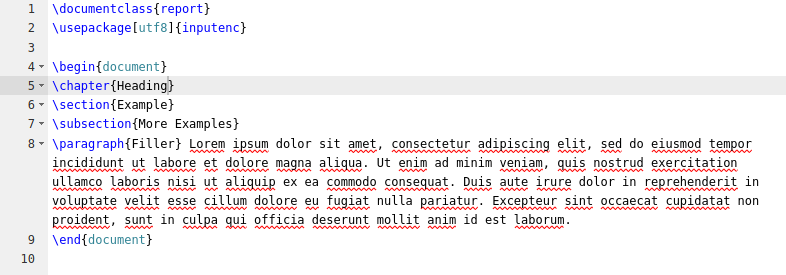
\includegraphics[scale=0.4]{img/LaTeX-Example-1.png}
    \caption{LaTeX document tags}
    \label{fig:my_label}
\end{figure}
\newpage
This code is then compiled and can be exported to a PDF to display like the following image.

\begin{figure}[h]
    \centering
    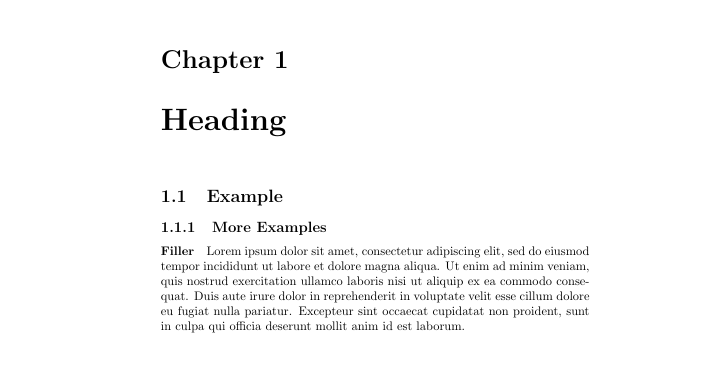
\includegraphics[width=1\textwidth]{img/LaTeX-Example-2.png}
    \caption{LaTeX output}
    \label{fig:my_label}
\end{figure}

LaTeX was the choice for our minor dissertation as we believed it was a clean and compact way of drafting up a document with the required structure put in place by our project supervisors. We were familiar with using it from a previous modules drafting documents such as literature reviews.

\section{Version Control}
\subsection{GitHub}

\begin{wrapfigure}{r}{1.5in}

\includegraphics[scale=0.7]{img/GitHub-Mark-120px-plus.png}
\caption{GitHub}
\cite{github}
\end{wrapfigure}
GitHub is a software hosting platform which allows users to collaborate and share their work. It contains social-network like functions where users can follow one another and view each others profiles. A user can readily find any number of projects in different stages in turn influencing their way of development of their own work\cite{vasilescu2015quality}.

This sole purpose of accessibility and versatility was the reason we used GitHub to share and collaborate on our project. It gave an in-depth breakdown of the changes made via commits, where we could see line-by-line what each member had completed or changed. This helped later when we merged each of our work together that we were working on separately making our whole experience with using GitHub extremely easy and satisfying.

\section{Integrated Development Environment}
\subsection{PyCharm}

\begin{wrapfigure}{r}{1.5in}

\includegraphics[scale=0.25]{img/PyCharm.png}
\caption{PyCharm IDE }
\cite{ide}
\end{wrapfigure}
PyCharm\cite{ide} is an Integrated Development Environment for the Python language developed by Jetbrains\cite{jetbrains}. Jetbrains are a software development company targeting many fields in the software community. Their products include plugins, programming languages, team tools and many IDE's. They provide IDE's for many languages like Java, C, C++, JavaScript etc. PyCharm is cross-platform with Windows, Apples Mac and Linux operating systems. With this IDE comes many useful features. These include support for web frameworks such as Django and Flask\cite{pycharm}, integration of version control for platforms like GitHub, support for scientific tools like numpy and scipy and simplistic code navigation via clean and concise user interface.

The decision to use PyCharm was an easy one amongst our team as it was an IDE that we have been using since the beginning of our third year of software development and similar to IDE's provided by Jetbrains like IntelliJ and WebStorm which we have been using since the beginning of our second year of software development. 

What we enjoy most about this IDE is it's simple and easy to use features\cite{pycharm}. Features such as the integrated version control for committing and pushing our project to GitHub and wide support for frameworks such as Django, which is our main framework for this project, proved to be vital in aiding in stress-free coding and teamwork.

\chapter{System Design}
This chapter details about how the above technologies are integrated into one system. It discusses each component in depth e.g. explaining how they link the system together. Diagrams and code snippets will be presented, where it is deemed relevant or necessary. These will hopefully offer a better understanding of the application. This application uses a 3-tier architecture similar to to MVC. These layers are: Data Tier, Logic Tier and Presentation Tier

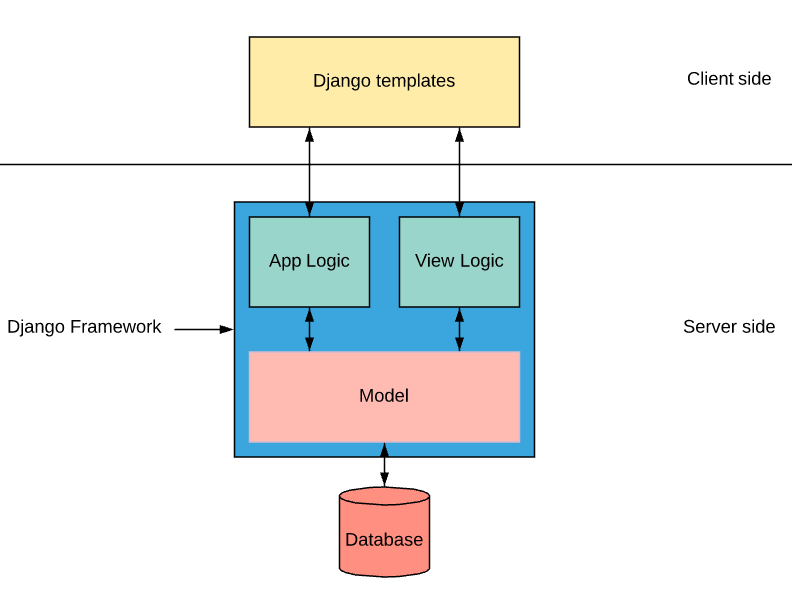
\includegraphics[scale=0.4]{img/uml.png}

\section{Design Overview}
The Presentation tier uses Django. This is a python-based framework. This will run the requests of the client through a process, in which, the request is sent down to the Logic tier to let the code written deal with the request. If the request is manipulating the database in any way, the request is sent down to the Data tier. In this case, the application is using SQLite.
\section{Data Tier}
When using databases for your application, it is important to choose one that works well with your desired framework. For this application, that ended up being SQLite. This was because of the reliability of the database as well as the speed of the querying to the tables themselves. To add the ability to access to table, we add this snippet of code to the settings.py file:
\begin{verbatim}
    DATABASES = {
    'default': {
        'ENGINE': 'django.db.backends.sqlite3',
        'NAME': os.path.join(BASE_DIR, 'db.sqlite3'),
        }
    }
\end{verbatim}
This will allow the table to access the database to perform all the CRUD functionality: create, read, update and delete. 
\section{Schema}
Before we can make any changes to the database, we have to define the structure of the database. This will allow us to define the attributes of each table. The tables were designed with functionality and security as the main focus. 
\subsection{store\textunderscore product}
This is where the entries for products added to the database are entered in. Here is a brief explanation of the structure of the database along with some of the choices made in the design phase
\subsubsection{id}
This is the ID of the product. It an integer(whole number) that must be unique. This is the optimal way to find a product for CRUD operations. This is used to specify a particular product. The admin doesn't set this number. It's an automatically-incremented number. So the ID of each object will be 1 greater than the ID of the previously created product. This is the primary key of the table since it is unique.
\subsubsection{name}
This is the name of the product. It is stored as a varchar which is a variable character field. It is set to length 200. This doesn't have to be unique
\subsubsection{price}
This is the price of the product. It is stored as a decimal since prices are rarely stored in integer format, they mostly have 2 decimal places. This is usually done to entice a consumer into buying with the illusion of a cheaper product. A good example is 4.95, 4.50 or 4.99
\subsubsection{size}
This is the size of the product. It is stored as a varchar of size 1 since all the products sold will be in single-letter sizes(small, medium and large).
\subsubsection{quantity}
This is the amount of this item left in stock. It is stored is an int because the amount has to be a whole number. For example, you can't have 5.5 of a particular clothing item in stock and also, the amount in stock cannot be negative.
\subsubsection{image}
This is the image of the actual product. It is stored on the database as a BLOB. A BLOB is a binary large object and can be up 2,147,483,647 characters long. It can hold up to 4 gigabytes of data. We chose BLOBs because our research had show that it would be the the optimal/only way to store images.

Name, size and price have to be populated but quantity and image can be left as NULL.

\begin{verbatim}
create table store_product
(
    id       integer      not null
        primary key autoincrement,
    name     varchar(200) not null,
    price    decimal      not null,
    size     varchar(1)   not null,
    quantity integer,
    image    blob
);
\end{verbatim}

\subsection{auth\textunderscore user}
This is the database for the users. It holds both, the administrators and the consumers. Here is a brief explanation of the structure of the database along with some of the choices made in the design phase
\subsubsection{id}
This is the ID of the user. The admin doesn't set this number. It's an automatically-incremented number. So the ID of each object will be 1 greater than the ID of the previously created product. This is the primary key of the table since it is unique.
\subsubsection{password}
This is the password that the associated user will need to log in to the app. The password isn't stored as it is entered. It is hashed before it is put in the database.
\subsubsection{last\textunderscore login}
This piece of information stores the last time this particular user logged in as a datetime variable. It is unused in this app
\subsubsection{is\textunderscore superuser}
This is a Boolean value that determines whether the user has access to the admin panel as well as some additional features added to the app.
\subsubsection{username}
This entry is for the username. It cannot be NULL and it has to be unique
\subsubsection{first\textunderscore name and last\textunderscore name}
These are varchar entries for the forename and surname of the user. They cannot be NULL and don't have to be unique
\subsubsection{email}
This is a varchar entry for the user's email. It cannot be NULL and doesn't have to be unique.
\subsubsection{is\textunderscore staff}
This is a Boolean value that determines whether the user has access to the admin panel as well as some additional features added to the app. This isn't used in this app since it is on the smaller end of the scale and doesn't require the use of staff
\subsubsection{is\textunderscore active}
This is a Boolean value that determines whether the user's account will still have the ability to access the app. This value may be changed if a user were to break guidelines.
\begin{verbatim}
create table auth_user
(
    id           integer      not null
        primary key autoincrement,
    password     varchar(128) not null,
    last_login   datetime,
    is_superuser bool         not null,
    username     varchar(150) not null
        unique,
    first_name   varchar(30)  not null,
    email        varchar(254) not null,
    is_staff     bool         not null,
    is_active    bool         not null,
    date_joined  datetime     not null,
    last_name    varchar(150) not null
);
\end{verbatim}

\section{Logic Tier}
This is seen as the middle-ground between the Data Tier and Presentation Tier. This is where the models and views are created.
\subsection{models.py}
This is where we outline the models of the classes to be used in the app. In this project, we use Product and User. It outlines the structure of these classes.

The Product layout is as follows:
\begin{verbatim}name = models.CharField(max_length=30)\end{verbatim}
No product name can go over 30 characters.
\begin{verbatim}price = models.DecimalField(max_digits=6, decimal_places=2)\end{verbatim}
No product can go over 9999.99.
\begin{verbatim}size = models.CharField(max_length=1, choices=SHIRT_SIZES)\end{verbatim}
Size is selected with a drop-down.
\begin{verbatim}quantity = models.IntegerField(default=0)\end{verbatim}
Quantity must be a positive, whole number.
\begin{verbatim}image = models.ImageField(upload_to="product_image", blank=True)\end{verbatim}
An ImageField can only be used with the installation of Pillow. This field can be NULL or blank. Images uploaded will be sent to the product\textunderscore image file in the media directory.

The User layout is as follows:
\begin{verbatim}
username = models.CharField(
    _('username'),
    max_length=150,
    unique=True,
    help_text=_('Required. 150 characters or fewer. Letters, digits and 
    @/./+/-/_ only.'),
    validators=[username_validator],
    error_messages={
        'unique': _("A user with that username already exists."),
    },
)
first_name = models.CharField(_('first name'), max_length=30, blank=True)
last_name = models.CharField(_('last name'), max_length=150, blank=True)
email = models.EmailField(_('email address'), blank=True)
is_staff = models.BooleanField(
    _('staff status'),
    default=False,
    help_text=_('Designates whether the user can log into this admin site.'),
)
is_active = models.BooleanField(
    _('active'),
    default=True,
    help_text=_(
        'Designates whether this user should be treated as active. '
        'Unselect this instead of deleting accounts.'
    ),
)
date_joined = models.DateTimeField(_('date joined'), default=timezone.now)
\end{verbatim}
These are all the default settings for User in Django. These values were not altered.

\subsection{views.py}
These are the methods that initially deal with the requests from the client side. The home page of the app is the index which is a list of all available products for sale. The URL for this is "/" meaning there is nothing after the domain name. For example, during development, this would have been "127.0.0.1:8000/". From there, there is a range of buttons and links. These are all associated with a view function. This means if the request sent to the view is a GET, it will usually render a HTML page. If this request was a POST however, it would mean data is being submitted and will be processed to make an alteration to the table.
\subsubsection{product\textunderscore view}
This takes 2 parameters; request and pk. Request holds to value of the datatype passed to it. In this case, it's either GET, POST or DELETE. Pk is an abbreviation of primary key. This is the optimal way to find a product since the primary key is unique. The pk for Product is id.
To ensure we are working with the correct product, we grab the product with the matching id(sent from the HTML) and call it product. We add this product to a dictionary called context.
If the request method is GET, return the details page for the product.
If the request method is GET with an edit appended to it, return the edit page for the product.
If the request method is POST, alter the values of that table entry with the values passed back from the HTML page, then save that product with it's new values.
If the request method is DELETE, remove that entry from the table.
\begin{verbatim}
def product_view(request, pk):
    product = Product.objects.get(pk=pk)
    context = {"product": product}
    if request.method == "GET":
        if request.GET.get("edit") is not None:
            return render(request,
            'store/product/edit_product.html.jinja2', context)
        else:
            return render(request, 'store/product/detail.html.jinja2', context)

    elif request.method == "POST":
        keys = ('name', 'size', 'price', 'quantity')
        if all((key in request.POST for key in keys)):
            for key in keys:
                setattr(product, key, request.POST[key])
            try:
                # product.image = request.POST['image']
                product.save()
            except ValidationError as e:
                context["notifications"] = []
                #add validation
                # print(e)
                context["notifications"].append("Validation Error")
                return render(request,
                'store/product/edit_product.html.jinja2',context)
            return render(request,
            'store/product/detail.html.jinja2', context)

    elif request.method == "DELETE":
        if product is not None:
            product.delete()
        return redirect(index)
\end{verbatim}
\subsubsection{add\textunderscore product}
This takes 1 parameter; which is request. Request holds to value of the datatype passed to it. This doesn't take a pk parameter since the product you are creating does not an id yet because it does not exist yet.
If the request method is GET, return the page for to create a new product entry.
If the request method is POST, create a new table entry with the values passed back from the HTML page and auto-create it's id.
\begin{verbatim}
def add_product(request):
    if request.method == "GET":
        return render(request, 'store/product/add_product.html.jinja2')
    elif request.method == "POST":
        keys = ('name', 'size', 'price', 'quantity')
        if all((key in request.POST for key in keys)):
            product = Product.objects.create(**{key:
            request.POST[key] for key in keys})
            product.save()
            return redirect(product_view, pk=product.pk)
\end{verbatim}
\subsubsection{view\textunderscore user}
This takes 1 parameter; which is request. Request holds to value of the datatype passed to it. This doesn't take a pk parameter since each session can only have 1 user.
If the request method is GET, return the details page for the user.
If the request method is GET with an edit appended to it, return the edit page for the user.
If the request method is POST, alter the values of that table entry with the values passed back from the HTML page, then save that user with it's new values.
\begin{verbatim}
def view_user(request):
    # user = User.objects.get(username=request.session.username)
    if request.method == "GET":
        if request.GET.get("edit") is not None:
            return render(request, 'customers/edit_user.html.jinja2')
        else:
            return render(request, 'customers/view_user.html.jinja2')
    elif request.method == "POST":
        user = User.objects.get(pk=request.user.pk)
        # if request.POST['username'] == User.objects.get(user.username):
        user.username = request.POST['username']
        user.first_name = request.POST['first_name']
        user.last_name = request.POST['last_name']
        user.email = request.POST['email']
        user.save()
        return redirect(view_user)
\end{verbatim}
\subsubsection{index}
This view only has a GET method which returns the main page. This is called from the urls.py file since the index is located at "/"
\subsubsection{login\textunderscore view}
If the request method is POST, take the values for username and password passed down from the HTML and use the authenticate method which takes the request and credentials and tests is user login information is valid and correct.
If the credentials are correct, log the user in and take them to the home page.
If the credentials are incorrect, ask for information again. Login attempts are unlimited.
If the request method is GET, return the login page to allow users to login.
\begin{verbatim}
def login_view(request):
    if request.method == 'POST':
        username = request.POST['username']
        password = request.POST['password']

        user = authenticate(request, username=username, password=password)
        if user is not None:
            login(request, user)
            return redirect('list')
        else:
            return redirect('login')

    elif request.method == 'GET':
        return render(request, 'registration/login.html.jinja2')    
\end{verbatim}
\subsubsection{register}
If the request method is POST, take the values for a new user passed down from the HTML, there are variables password and password2. If password and password2 are the same value, create a new entry into the table.
If the request method is GET, return the register page to allow users to register.
\begin{verbatim}
def register(request):
    if request.method == 'POST':
        print(request.POST.keys())
        username = request.POST['username']
        password = request.POST['password']
        first_name = request.POST['first_name']
        last_name = request.POST['last_name']
        email = request.POST['email']
        password2 = request.POST['password2']

        if password == password2:
            user = User.objects.create_user(username=username,
            password=password, 
            first_name=first_name,
            last_name=last_name, email=email)
            user.save()
            user = authenticate(request, username=username, password=password)
        else:
            redirect(index)

        if user is not None:
            login(request, user)
            return redirect('view_user')

        else:
            return redirect('login')

    elif request.method == 'GET':
        return render(request, 'registration/register.html.jinja2', {})    
\end{verbatim}
\subsubsection{logout}
Logout is used to log the user out by clearing the session and then returns the home page.
\subsubsection{cart}
The cart is a collection of items that had their "add to cart" button clicked on the HTML pages.
If the request method is GET, the view finds cart in the HTML and then an empty array called products. If the cart exists, it creates a list which filters to pull out the integers. These integers are product ids. These are in the cart from the POST method. It compares all these numbers against the product ids to find the names of the products. If the product exists, it is added to the products array. This is all returned as JSON data instead of a separate HTML page.
If the request method is POST, this means the "add to cart" or "remove from cart" buttons have been clicked. The view takes in the id of the product that the button was clicked on. It takes this id and checks that is both numeric and populated. If the product exists, the cart is retrieved. This is in anticipation of changes to the cart. If the action is "add to cart", the item is added to cart. If the action is "remove from cart", the item is removed from cart. The session pf the cart is then updated.
\begin{verbatim}
def cart(request):
    if request.method == 'POST':
        action = request.POST.get("action", None)
        if action == "add_to_cart" or action == "remove_from_cart":
            product_id = request.POST.get("product_id", None)
            if product_id is not None and product_id.isnumeric():
                product = Product.objects.get(pk=product_id)
                if product is not None:
                    cart = str(request.session.get("cart", "")).split(",")
                    if action == "add_to_cart":
                        cart.append(product_id)
                        product.quantity -= 1
                    else:
                        cart.remove(product_id)
                        product.quantity += 1
                    request.session["cart"] = ",".join([i for i in cart if i != 
                    ""])
                    return HttpResponse(status=200)
                else:
                    return HttpResponse(status=404)
            else:
                return HttpResponse(status=400)
        else:
            return HttpResponse(content="unknown action", status=400)
    elif request.method == 'GET':
        cart = request.session.get("cart")
        products = []
        if cart is not None:
            cart = list(filter(str.isnumeric, cart.split(",")))
            for product_id in cart:
                product = Product.objects.get(pk=product_id)
                if product is not None:
                    products.append(product)

        return HttpResponse(content=serializers.serialize('json', products), 
        content_type='application/json')
    
\end{verbatim}

\section{Presentation Tier}
This is the part of the application that the average user will interact with. The main part people associate with the front-end is the graphical user interface but there is still a lot of logic associate with presenting carefully sculpted data to the user. This project uses Jinja2, Javascript and CSS.
\subsection{Base Page}
This page is the base of most consumer usable pages. It holds the cart, a notifications panel and a footer for login, logout and register. It also contains the script for manipulation and presenting the cart. 
The addToCart and removeFromCart functions just call their respective functions in the POST method of the cart view. 
updateCart calls the GET method from the cart view. This is called every time a page that extends cart is loaded. It is also called every time a change is made to the cart itself by using them "add to cart" button or "remove from cart" button. It creates a list for presenting each product entry. The name and price of the item are added to the list through each iteration. At the ended, the total of all the products is displayed. 

\section{Password Hashing}
By default, Django hashes all passwords. It does this using the PBKDF2 algorithm along with a SHA256 hash to extend the length of the password. This, in return, takes far more time to break.
\begin{verbatim}<algorithm>$<iterations>$<salt>$<hash>\end{verbatim}
These are the steps used to store a password in Django. These steps are separated by the dollar signs. 
\begin{verbatim}<algorithm>\end{verbatim} represents the algorithm used. In this case, it is PBKDF2.
\begin{verbatim}<iterations>\end{verbatim} is the amount of times the algorithm acts on the test subject. In this case, it's 180000 times.
\begin{verbatim}<salt>\end{verbatim} represents the random salt added to the end of the string before it is hashed. It is done by calling the function \begin{verbatim}get_random_string()\end{verbatim}
\begin{verbatim}<hash>\end{verbatim} then returns the result which will be the string stored as a password in the database.

\chapter{System Evaluation}
This will discuss the tests carried out on the application throughout the development and when development finished. This was all done to ensure the best product possible was created.
\section{Testing Overview}
Testing is very important to any application. It can aid the development cycle by point out system flaws or bugs or hardware drawbacks. It is recommended that applications go through the following tests:
\subsection{Unit Testing}
Unit testing is carrying out tests on individual components of the application to ensure that they can all carry out their allocated tasks. The front-end unit testing was carried out by doing out own tests manually and we also used the Firefox plugin tool called Selenium for automated tests. Server-side unit testing was carried out using Postman. We manually compared the results to what they should be. Unit testing can provide full code coverage so we were very happy with the results.
\subsection{Functional Testing}
Functional testing is carried out on whole functions throughout the app. These were carried out on the client-side manually by comparing the data sent by the admin to the data being displayed on the application. This was done by passing test data through the application in hopes of our desired results. All of our tests passed. This had full code coverage. 
\subsection{Usability testing}
We would show our project to our supervisor in each of our weekly meetings after development began. Newer features were presented to the supervisor along with the beginnings of the next step. We always took their advice on board in order to reach their expectations. We tried to implement every part we could. We tested usability by manually using the app ourselves as well as getting some friends and family members to use it. We took all constructive criticism on board.
\subsection{Integration Testing}
We carried out integration testing each time a new component was added. An example of this was testing the ability to display the user's data. This was done to make sure this specific component worked and didn't interfere with the functionality of the products or store. The inclusion of user data representation and manipulation left the product data unaffected.
\subsection{Security Testing}
Data protection is becoming increasingly important in today's world. We had to be sure that only the user would be able to see the data. If a system is tested more often, it will be far more secure. Test should start after the first component is implemented and regularly throughout the life cycle of the application development. The main principles of security are integrity, confidentiality, authentication and authorization. We made sure that consumers would not be able to access the admin panel if unauthorized. We made sure to hash every password so if the password was leaked from our side, the password would not work and would be basically impossible to reverse-engineer. Users and admins carry CSRF tokens throughout the app to keep the session secure. If a user doesn't have a token, they will get a 403(forbidden) error for most pages. Tests were also carried out with Postman to ensure that CSRF authentication tokens weren't distributed unnecessarily.
\subsection{Compatibility testing}
This application will have to be able to run on an endless amount of environments. It has to be able to run on any operating system or browser. We tested this application on Windows 10, Windows 7, Windows Vista, mac OS, Ubuntu, Fedora and Archlinux. We ran it on several browsers including: Chrome, Edge, Safari, Brave, Internet Explorer and Firefox. All returning desired results.
\subsection{Performance Testing}
Performance is very important to any application. How the project performs locally during development isn't always an indicator to how it will perform at a larger scale. We didn't feel the need to pay for our choice of performance testing. A lot of the free services were very lackluster in terms of features and testing intensity. After reading some reviews and considering ease of accessibility. We decided it may be better to use the free version of a paid service. The main types of tests are: endurance testing, load testing and scalability testing. We knew the scalability wouldn't be great due to the drawbacks of SQLite in the speed category. In terms of endurance testing, we were impressed. It showed that the app may have some longevity. It performed well in load testing, not being troubled by 100 requests per second for 1 minute.
\subsection{Acceptance Testing}
This was done by handing the product over to friends and family for testing to gauge how far away we were from a finished product. We found most feedback to be very useful. This helped us gain an insight to what the average customer wanted
\subsection{Limitations}
The main limitation of this project overall was time. Due to the COVID-19 pandemic, our schedule for submission changed for every project. Which left all the deadlines far more condensed at the end of the semester. This meant we never got around to adding a multitude of features we wanted to have, the main example being a checkout. A lot of time was taken up by designing our own views. Djago has it's own default templates and views but we felt it necessary to do our own. We felt this because, not only are the templates very basic, but they only need a few lines of code. This doesn't provide every feature we want and it also doesn't show you how the code works at all. We felt it would be far more worth while in the long doing our own. This wasn't a case of reinventing the wheel, it was more of a restructuring. Because of this, our code was left very different to any tutorials online. We may have fallen short on some functionality but we're very proud to say this is all completely our own code. This lack of time meant we couldn't implement such things as:
\begin{itemize}
    \item search and filter
    \item checkout
    \item password reset for users(can be done by request from an administrator)
    \item image upload(can be done with admin panel)
    \item a notifications panel that we had started but couldn't finish.
\end{itemize}

\chapter{Conclusion}
This conclusion will briefly discuss our entire project as a whole. We will be breaking down the project discussing our objectives we set out in our introduction chapter and if they were achieved. Outlining the objectives we set is crucial to us as it will determine whether this project as a whole was a success or failure. We will also be setting out what we learned over the course of this project and what skills we took away from development; using new languages or platforms or improving on existing languages.

\section{Objective set out to achieve}
In the beginning of our project planning and outlined at the start of our dissertation, setting baseline objectives was important as it created a main focus on what had to be completed. These objectives were outline in the introduction in \textit{Section 1.1} where we aimed for the following goals:

\begin{itemize}
\item Outline the basic concept of the project.
\item Understand the technologies used.
\item Detail of the development of the project.
\item Implement and explore new technologies use.
\item Design an aesthetically pleasing and simple website.
\item A collaborative effort between team-members to complete the project.
\end{itemize}

\subsection{Outline the basic concept of the project}
We believed that we clearly outlined the basic concept what our project is about and how we plan on going about creating it. In \textit{chapter 2, context}, we outlined what is involved in e-commerce web applications and provided examples of successful apps. We continued by breaking down the types business models available to e-commerce applications and why we chose these models. These models were successfully implemented into our project as it is a business-to-consumer as planned and described.

\subsection{Understand the technologies used}
In completing our project, we feel that the technologies we used were best suited for our chosen e-commerce web application. We explored the wide variety of technologies we could've chosen outlining why the one we picked was best suited. We feel that we concisely detailed this in our \textit{Methodology} chapter for the readers of our dissertation.

\subsection{Detail of the development of the project}
Throughout this dissertation, we believe that within each chapter we discussed, in great detail, how we went about developing our project and what software was necessary in completing it. This is clear in chapters like \textit{Methodology}, \textit{Technology Review} and \textit{System Evaluation} we broke the development of our project up and outlined in great detail what each part consisted of which we feel was comprehensive and accurate.

\subsection{Implement and explore new technologies used}
Throughout our development, we had discussed our choice of technologies and whether we wanted to be doing the usual angular application. With our initial plan including using technologies we were completely familiar with changing to that of technologies we had either never used or only limited experience in using, we believed that what we have learned in using and implementing these new technologies proved to be a great success. We take away with us the skills of each of these technologies that will hopefully hold great benefit in the future.

\subsection{Design an aesthetically pleasing and simple website}
In designing our project, we believed that we completed the goal of keeping our user interface aesthetic and simple to use. We kept the colour scheme simple and made sure it never conflicted at on any pages. This would appeal to the user when using the application in conjunction with easily navigable pages.

\subsection{A collaborative effort between team-members to complete the project}
In completing this project we found that the collaborative effort put in by both members helped complete the overall goals set out in this project. We worked very well as a team breaking down our project and effectively assigning the workload evenly. We stayed in regular contact with one another with frequent updates on what each of us were working on. Keeping in constant communication with one another was vital as it helped resolve any issues that arose swiftly.

\section{Learning outcomes}
We feel we have learned a great deal, not only about Django, but about frameworks in general. It gave us a far better understanding of how a regular web app works. This showed us how apps deal with GET and POST requests and URL directions. It also gave us a far better understanding of how application use views and/or controllers to manipulate data to give the desired result to the consumer. We had to learn a lot about HTML and session logic which is very important for the final product. We delved deeper than we ever have before into CSS to get the application to look as sleek and consistent as possible. We also had to use JavaScript which we had used very sparingly before this project.
\newpage
\section{Reflection}
This conclusion is brought to an end with a few words from each member of this project and their thoughts.
\subsection{Niema Attarian}
I thoroughly enjoyed developing this project. Being an avid user of endless online shopping websites this was something Mark and I were determined to do out and design. Working with Mark was as expected; easy and stress-less. We have been close friends since our first year of Software Development in G.M.I.T so it was an absolute pleasure to have worked with him. I would also like to thank our project supervisors Gerard Harrison, who has been exceptional in giving us endless advice and holding meetings to discuss our project and Dr. John Healy who has been so supportive over our four years of college.
\subsection{Mark Gill}
I very much enjoyed my experience with this project and it is something I could see being continued throughout the Summer. I was very happy to be given the chance to pair up with Niema since we have been friends since the start of the college course. We both were on the same train of thought in terms of project ideas and I found very hospitable and easy to work with throughout the life cycle of the project. I would like to sincerely thank our supervisors: our group supervisor, Gerard Harrison and and our year supervisor, Dr. John Healy for the part they played in the project which finished off a very enjoyable and rewarding 4 years in GMIT.

\chapter{Appendices}

\subsubsection{GitHub Project Source code}

\textit{Niema Attarian:} \href{https://github.com/niemaattarian/Final-Year-Project}{https://github.com/niemaattarian/Final-Year-Project}
\newline
\textit{Mark Gill:} \href{https://github.com/markgill17/Final-Year-Project}{https://github.com/markgill17/Final-Year-Project}

\subsubsection{Deployment Link}
\textit{Link:} http://167.99.86.212/

\subsubsection{Screencast Video}
\textit{Link:} https://youtu.be/Qavgu-KkZTc

  \bibliographystyle{ieeetr}
  \bibliography{bibliography}
\end{document}